\section{Deep Learning Optimizations}
\begin{itemize}
	\item Pure optimization has a very direct goal, namely finding the optimum. However, in Machine Learning, we want to not only make small errors on training data but also generalize well to new data. Thus, the "optimal" parameters might not necessarily be the optimum (e.g. overfitting)
\end{itemize}
\subsection{Stochastic Gradient Descent}
\begin{itemize}
	\item Pushing the weights towards highest gradient change
	$$w_{t+1} = w_{t} - \eta_t \nabla_{w} \mathcal{L}$$
	\item \textit{(Batch) Gradient descent}: gradients on the full dataset. However:
	\begin{itemize}
		\item Dataset is mostly too large for this
		\item No real guarantee that this leads to a good optimum and/or it will converge faster
	\end{itemize}
	\item \textit{Stochastic gradient descent}: approximate gradients from random mini-batch. 
	\begin{itemize}
		\item Standard error is inverse proportional to number of elements $m$ in a batch: $\sigma / \sqrt{m}$, where $\sigma$ is variance in $p(x,y^*)$
		\item Noisy gradients help to escape local minima, acts as regularization, reduce overfitting (good shuffling important)
		\item Does sample roughly representative gradients from dataset. Is better as training data is also just a rough approximation of what the test data might look like (optimum on training $\neq$ optimum on test)
		\item SGD is faster, especially in first iterations
		\item SGD is able to adapt with dynamically changing datasets (and also good for streaming data)
		\item make sure of class/data balance in batches
	\end{itemize}
	\item \textit{Ill conditioning}: if gradients are large, applying them can lead to worse performance. This is the case if the second order derivative changes faster 
\end{itemize}
\begin{figure}[ht!]
	\centering
	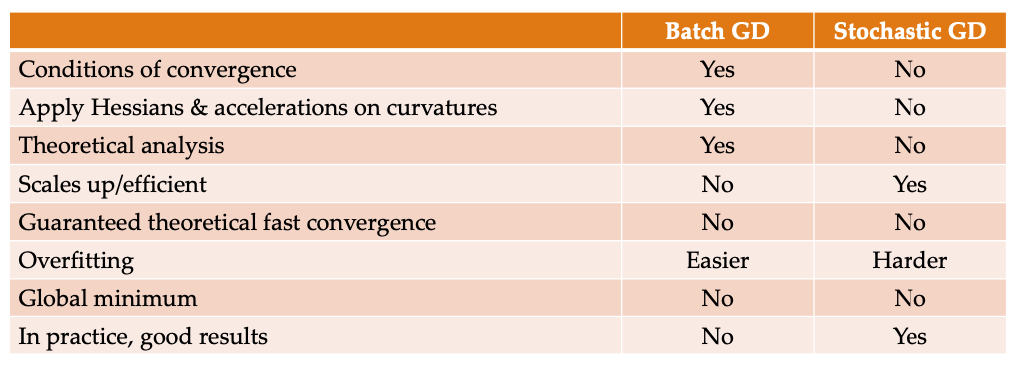
\includegraphics[width=0.7\textwidth]{figures/SGDvsGD.png}
	\caption{SGD vs GD}
	\label{fig:SGDvsGD}
\end{figure}
\subsection{Advanced optimizations}
\subsubsection{Gradient-based optimization}
\begin{itemize}
	\item \textit{Pathological curvatures}: move through a ravine towards minimum. SGD tends to oscillate between the walls because they have high gradients
	\begin{itemize}
		\item Second order optimization can help a lot for pathological curvatures: $$w_{t+1} = w_{t} - H_{\mathcal{L}}^{-1} \eta_t g_t$$
		\item Hessian $H_{\mathcal{L}}^{ij} = \pd{\mathcal{L}}{w_i\partial w_j}$ works as adaptive learning rate per parameter
		\item However, unfeasible in practice because Hessian gets very large
	\end{itemize}
	\begin{figure}[ht!]
		\centering
		\includegraphics[width=0.3\textwidth]{figures/optimization_pathological_curvatures.png}
		\caption{Pathological curvature}
		\label{fig:optimization_pathological_curvatures}
	\end{figure}
	\item \textbf{Momentum}: maintain \textit{momentum} from previous parameter updates to dampen the oscillations.
	\begin{equation*}
		\begin{split}
			u_{t+1} & = \gamma u_{t} - \eta_t g_t \\
			w_{t+1} & = w_{t} + u_{t+1}
		\end{split}
	\end{equation*}
	\begin{itemize}
		\item Works as a exponential averaging $\Rightarrow$ more robust gradients, faster convergence
		\item $\gamma$ might be initialized lower and then increased over time to $0.9$
		\item Standard values for $\gamma$ are between $0.5$ and $0.9$ (note that a lower learning rate should be used compared to standard SGD)
	\end{itemize}
	\item \textbf{RMSprop}: adapting learning rate on current loss surface.
	\begin{equation*}
		\begin{split}
			r_t & = \alpha \cdot r_{t-1} + \left(1 - \alpha\right) \cdot g_t^2\\
			\eta_t & = \frac{\eta}{\sqrt{r_t} + \epsilon} \\
			w_{t+1} & = w_{t} - \eta_t \cdot g_t\\
		\end{split}
	\end{equation*}
	\begin{itemize}
		\item $r_t$ is the (exponentially) averaged gradient norm describing the size of the gradients (per dimension!)
		\item The learning rate is then adapted by $\eta_t$ at every time step for each dimension independently
		\item $\epsilon$ to prevent numerical instability and too large learning rates
		\item With the adapted learning rate, we update our weights with SGD
	\end{itemize}
	\item \textbf{Adam}: Combining adaptive learning rate and momentum
	\begin{equation*}
		\begin{split}
			m^{(t)} & = \beta_1 m^{(t-1)} + (1 - \beta_1)\cdot g^{(t)}\\
			v^{(t)} & = \beta_2 v^{(t-1)} + (1 - \beta_2)\cdot \left(g^{(t)}\right)^2\\
			\hat{m}^{(t)} & = \frac{m^{(t)}}{1-\beta^{t}_1}, \hat{v}^{(t)} = \frac{v^{(t)}}{1-\beta^{t}_2}\\
			w^{(t)} & = w^{(t-1)} - \frac{\eta}{\sqrt{v^{(t)}} + \epsilon}\circ \hat{m}^{(t)}\\
		\end{split}
	\end{equation*}
	\begin{itemize}
		\item Keeps track of the gradient norm for momentum $m^{(t)}$, and norm (also known as velocity) $v^{(t)}$
		\item The hyperparameters $\beta_1$ and $\beta_2$ correlate with the $\gamma$ and $\alpha$ respectively from the previous approaches
		\item The adaptive learning rate is expressed by $\hat{v}^{(t)}$, and the exponentially averaged gradients by $\hat{m}^{(t)}$
		\item The division is to remove the bias of $m^{(0)}$ and $v^{(0)}$ being zero. Note that $\beta_1^t$ means the value of $\beta_1$ to the power $t$, and not at time step $t$
		\item Adam is in general better for complex models, but might fail on easy/stupid tasks compared to simple methods like SGD
	\end{itemize}
	\item \textbf{Adagrad}: adapting learning rate based on both gradient scale and frequency of updates
	\begin{equation*}
		\begin{split}
			G_t & = G_{t-1} + \text{diag}\left(g_t^2\right)\\
			w_{t+1} & = w_{t} - \frac{\eta}{\sqrt{G_t + \epsilon}}\cdot g_t\\
		\end{split}
	\end{equation*}
	\begin{itemize}
		\item Very similar to RMSprop, but sums the scales over all time steps ($G_t$) instead of exponentially averaging 
		\item Less sensitive to learning rate tuning, but it gets very small over training time annealing to 0
	\end{itemize} 
	\item \textbf{Nesterov momentum}: use the future gradient instead of the current gradient. Leads to better convergence in theory
\end{itemize}
\subsubsection{Bayesian optimization}
\begin{itemize}
	\item Gradient-based optimizations have the problem of getting stuck in local minima
	\item Bayesian optimization is a gradient-free, educated trial and error guesser that works in lower dimensional spaces (up to 1000, but mostly 20 to 50 parameters)
	\item Determines the next point/parameter values to evaluate based on variance/uncertainty, and expected/predictive value. 
	\item Can be used for e.g. network architecture search
\end{itemize}
\subsection{Normalization}
\begin{itemize}
	\item Data pre-processing
	\begin{itemize}
		\item Center data around 0 (activation functions are designed for that)
		\item Scale input variables to have similar diagonal covariances (not if features are differently important)
		\item De-correlate features if there is no inductive bias (e.g. sequence over time)
	\end{itemize}
	\item \textbf{Batch normalization}: ensure Gaussian distribution of features over batches at every module input
	\begin{equation*}
		\begin{split}
			\mu_B = \frac{1}{m} \sum\limits_{i=1}^{m} x_i, &\hspace{5mm} \sigma_B^2 = \frac{1}{m} \sum\limits_{i=1}^{m} \left(x_i - \mu_B\right)^2 \\
			\hat{x}_i & = \frac{x_i - \mu_B}{\sqrt{\sigma^2 + \epsilon}} \\
			\hat{y}_i & = \gamma \cdot \hat{x}_i + \beta
		\end{split}
	\end{equation*}
	\begin{itemize}
		\item Normalize feature to $\hat{x}_i \sim \mathcal{N}(0,1)$, then rescale with trainable parameters $\gamma$ (variance) and $\beta$ (mean).
		\item Helps the optimizer to control mean and variance of input distribution, and reduces effects of 2nd order between layers $\Rightarrow$ easier, faster learning 
		\item Acts as regularizer as distribution depends on mini-batch and therefore introduces noise
		\item During testing, take a moving average of the last training steps and use those for $\mu_B$ and $\sigma_B^2$
	\end{itemize}
\end{itemize}
\subsection{Regularization}
\begin{itemize}
	\item Weight regularization needed to prevent overfitting
	\item \textbf{$\ell_2$-regularization}: Introduce objective term for minimizing weights
	$$w^{*}=\arg\min_w \mathcal{L} + \frac{\lambda}{2}\sum_l ||w_l||^2$$
	\begin{itemize}
		\item When using simple (stochastic) gradient descend, then $\ell_2$ regularization is the same as weight decay: $$w_{t+1} = \left(1-\lambda \eta_t\right) w_{t} - \eta_t \nabla_{\theta} \mathcal{L}$$
	\end{itemize}
	\item \textbf{$\ell_1$-regularization}: use $\ell_1$ objective, introduces sparse weights
	$$w^{*}=\arg\min_w \mathcal{L} + \lambda \sum_l ||w_l||$$
	\item \textbf{Early stopping}: stop the training when test error increases but training loss continues to decrease. Can be counted to regularization as training steps are reduced
	\item \textbf{Dropout}: setting activations randomly to 0 during training with probability $p$ (mostly between $0.1$ and $0.5$)
	\begin{itemize}
		\item During test time, every activation is reweighted by $1 - p$
		\item Reduces co-adaptations/-dependencies between neurons because none can solely depend on the other
		\item Neurons get more robust $\Rightarrow$ reduces overfitting
		\item Effectively, a different network architecture is used every iteration. Testing can be seen as using model ensemble
	\end{itemize}
\end{itemize}
\subsection{Weight initialization}
\begin{itemize}
	\item There are two forces on the weight magnitude: small weights are needed to keep data around origin, but large weights are required to have strong learning signals
	\item Initialization should preserve variance of activations (input variance $\approx$ output variance to keep distribution between modules same)
	\item Depends on non-linearity and data normalization
	\item \textbf{Xavier initialization}: to maintain data variance, the variance of the weights must be $1/d$ where $d$ is number of input neurons $\Rightarrow$ sample weight values from $w\sim\mathcal{N}(0,\sqrt{1/d})$
	\item \textbf{Initialization for ReLU}: ReLU set half of the output neurons to 0 $\Rightarrow$ double the weight variance to compensate zero flat-area: $w\sim\mathcal{N}(0,\sqrt{2/d})$
\end{itemize}